\documentclass[11pt, oneside]{article} 
\usepackage{geometry}
\geometry{letterpaper} 
\usepackage{graphicx}
	
\usepackage{amssymb}
\usepackage{amsmath}
\usepackage{parskip}
\usepackage{color}
\usepackage{hyperref}

\graphicspath{{/Users/telliott_admin/Tex/png/}}
% \begin{center} 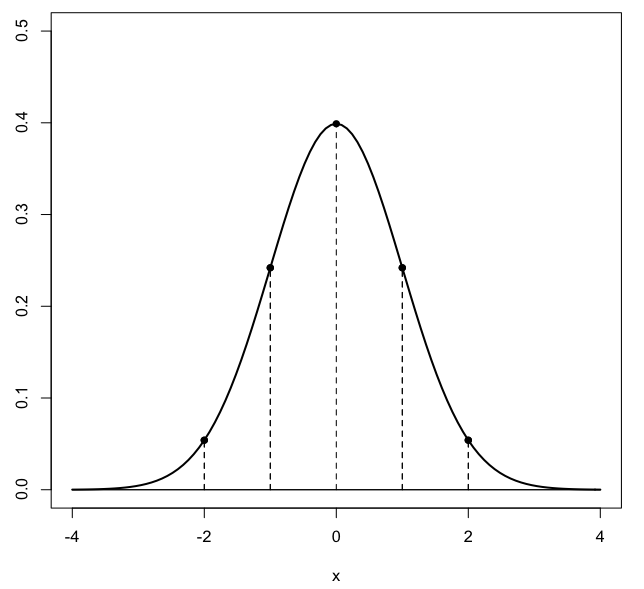
\includegraphics [scale=0.4] {gauss3.png} \end{center}

\title{Easy pieces}
\date{}

\begin{document}
\maketitle
\Large

\hypertarget{first_calculus}{}
As an example of the two fundamental ideas in calculus, refer to the instruments one uses while driving a car. Most good drivers look regularly at the speedometer, which measures velocity, or how fast you're going.  

On the other hand, if someone gives you directions:  "go 3 miles past the gas station and then turn left", you will want to know about distance covered and check the odometer.

\begin{center} 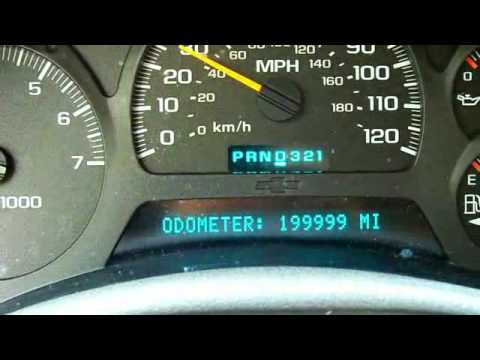
\includegraphics [scale=0.5] {hqdefault.jpg} \end{center}

Velocity is the \emph{rate of change} of distance with time, distance divided by time.  In other words, velocity times time equals distance.  (We can think of speed and velocity as the same for now.)

In calculus we say that the velocity is the \textbf{derivative} of the distance with respect to time, and the distance is the \textbf{integral} of the velocity with respect to time.  The latter must be evaluated between starting and stopping points for the time, as we'll see.

\subsection*{time-dependence}
Distance equals velocity times time.

This is easy if the velocity is a constant.  Travel at $60$ miles per hour for $2$ hours and you'll go $120$ miles.  It is standard to use $s$ to refer to the distance traveled and $v$ for velocity.  If the velocity is constant then:
\[ s = vt \]

Suppose we plot velocity as a \emph{function of time} ($v$ on the $y$-axis and $t$ on the $x$-axis).

\begin{center} 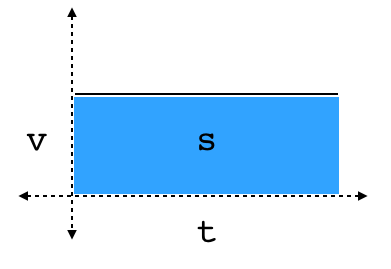
\includegraphics [scale=0.5] {velocity_time1.png} \end{center}

If the velocity is constant, then we obtain a straight horizontal line.  Furthermore, the distance traveled is the \emph{area under the curve} (and above the $x$-axis) which is the area of a rectangle with sides $v$ and $t$ and as we said $s = vt$.

However, for the most interesting problems velocity is not constant.  

For a car, imagine increasing the pressure on the gas pedal steadily so that, starting from a stop at zero time, after $1$ second you are going $10$ mph, after $2$ seconds $20$ mph, after $3$ seconds $30$ mph. If we continue at the same rate, we'll accelerate from $0$ to $60$ mph in $6$ seconds, quite a respectable time.

This is constant acceleration.

We say that $v$ is a constant function of time, and we can write 
\[ v = at \]
where $a$ is the acceleration.

\begin{center} 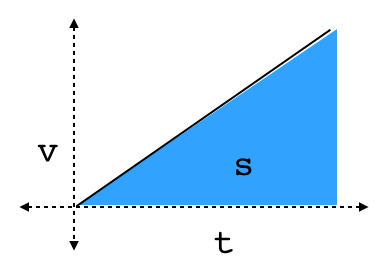
\includegraphics [scale=0.5] {velocity_time2.png} \end{center}

If $a$ is not zero then $v$ changes with time.  If $a$ is non-zero and constant, then $v$ changes at a constant rate.  Starting from $v=0$, the final velocity will be $v = at$, but the distance traveled is not 
\[ s = vt \stackrel{?}{=} at^2 \]

For variable velocity, the distance traveled is the \emph{average} velocity times the time.  For smooth (constant) acceleration from zero to $v$, the average velocity is
\[ v_{\text{avg}} = \frac{v}{2} \]

So the correct equation is:
\[ s = v_{\text{avg}}\ t  = \frac{1}{2} v t \]
and since $v = at$
\[ s = \frac{1}{2} at^2 \]

In this case, if we plot velocity as a function of time, we obtain a straight line that extends diagonally up with respect to the $x$-axis.  The distance traveled is the area under the curve (below the line and above the $x$-axis).  

The shape whose area is needed is a triangle.  This also accounts for the factor of $1/2$.

You probably know that if a mass $m$ is dropped from a tall building like the Tower of Pisa, then the distance it has fallen goes like the square of the time.  The correct equation is (again):

\[ s = \frac{1}{2} g t^2 \]
where $g$ is the acceleration due to gravity.  Usually we consider this acceleration as negative, and the distance traveled has the same sense.

Galileo knew this equation, which he obtained not from experiments at the Tower of Pisa, but by timing the descent of balls down an inclined plane.

\subsection*{detail}

If you want to be more complete and say that the starting point is not necessarily the origin of the coordinate system, add a constant $s_0$ to describe the initial distance from the origin and obtain:
\[ s = vt + s_0 \]
and similarly, a constant $v_0$ to describe the initial velocity as shown above.

In fact, the full equation of motion is 
\[ s = \frac{1}{2} a t^2 + v_0 t + s_0 \]

We'll say much more about this later.

\subsection*{simple rules}

We will introduce the theory of calculus a bit more formally in the next section of the book.  For now, let's just talk about a simple rule.

Switching notation to $y$ and $x$, we have that $y$ is a function of $x$.  We write $y = f(x)$, and list three types of dependency:

\[ y = c \]
\[ y = cx \]
\[ y = cx^2 \]

 (with $c$ as a constant.)
 
We ask "what happens if we change $x$ a little bit?"  We call this little bit of $x$, $dx$.  

What happens to $y$?  $y$ also changes by a small amount.  Call that amount $dy$.

In the first case $y = c$, $y$ does not depend on $x$ at all.  The result is zero.
\[ y = c \]
\[ dy = 0 \cdot dx \]

Rewrite this as:
\[ \frac{dy}{dx} = 0 \]

The ratio $dy/dx$ is the slope of the curve formed by plotting $y$ against $x$.  We call that the derivative of the function $f(x)$.

This plot is a horizontal line with slope $m = 0$.

In the second case, $y$ is a linear function of $x$, so the change in $y$ is the change in $x$ multiplied by $c$:
\[ y = cx \]
\[ dy = c \cdot dx \]
We can also rewrite this as 
\[ \frac{dy}{dx} = c \]

In analytical geometry, we calculate the slope of a line as $\Delta y/\Delta x$, and it's important that for a line, the slope is constant and so it doesn't matter which values $x_1,x_2,y_1,y_2$ we choose for the calculation
\[ m = \frac{\Delta y}{\Delta x} = \frac{y_2 - y_1}{x_2 - x_1} \]

Above we had the example where $v = at$.  Then $dv/dt = a$.

In the third case we have
\[ y = cx^2 \]

For a parabola, the slope of the curve at a point (what's called the tangent to the curve $y = cx^2$) really does depend on the choice of $x_1,x_2,y_1,y_2$.  The slope is steeper the further out you go in a positive direction on the $x$-axis.

The key insight is that if $x_1$ is sufficiently close to $x_2$ the slope is constant.  It's like saying that the earth is flat \emph{locally}.  If you detect any curvature, just zoom in a bit and ask an ant --- the earth is definitely flat for Flik.
\begin{center} 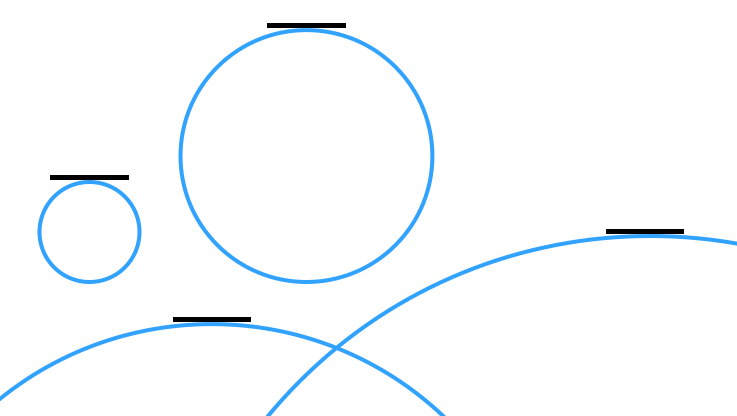
\includegraphics [scale=0.5] {line_circles.png} \end{center}
In the figure above, the line has constant length, but the distance to the circle from the middle of the line decreases as we increase the size of the circle.

Even if we are accelerating in the car, we have a unique velocity at a particular instant in time.

Put yet another way, for a very small change $\Delta x$ in either direction from $x$, we can get the same slope:
\[ m = \frac{y + \Delta y}{x + \Delta x} = \frac{y - \Delta y}{x - \Delta x}  \]
We get the same slope -- \emph{if} $\Delta x$ is small enough.  But if it's not, we can always make it smaller.  That's the beauty of the real numbers.

Since the changes $\Delta x$ and $\Delta y$ are very small, and in theory \emph{approach} zero in the limit, we use the new nomenclature:  $dy$ and $dx$.

For the parabola, we apply the power rule, which says that the derivative is
\[ \frac{dy}{dx} = 2cx \]

Applied to the equation of motion under gravity
\[ s = \frac{1}{2} a t^2 + v_0 t + s_0 \]
\[ v = \frac{ds}{dt} = at + v_0 \]
\[ \frac{dv}{dt} = a \]

The general form of the power rule is that if
\[ y = x^n \]
then
\[ \frac{dy}{dx} = n x^{n-1} \]

For example, if $y$ depends on $x^3$ like
\[ y = cx^3 \]
then
\[ \frac{dy}{dx} = 3cx^2 \]

This rule had already been discovered before Newton (it's a toss-up whether Fermat or Cavalieri was first).

We call the derivative $dy/dx$ the slope of the curve $y = f(x)$.  Recall that for standard analytical geometry, the slope is $\Delta y/\Delta x$.  For a straight horizontal line, the slope is zero.  For a line $y = mx + b$, the slope is $m$.

This brings up another small point, namely that the derivative of a polynomial like $mx + b$ is the sum of the derivatives of each term.

\subsection*{integration}

Now, we boldly claim that from the point of view of problem-solving, integration is the reverse (or inverse or converse) of differentiation.  Mathematicians hate this kind of statement, because it trivializes what is a profound statement, the fundamental theorem of calculus.  

But for problem-solving we claim that this \emph{doesn't matter}.

Take the example above:

 \[ \frac{dy}{dx} = 3cx^2 \]
Put the $dx$ on the right-hand side:
\[ dy = 3cx^2 \ dx \]

What this says is that for a small change in $x$ called $dx$, we obtain a small change in $y$ called $dy$ with the given relationship.

To find the total change in $y$ for a change in $x$, we integrate.  Integrals contain the symbol $\int$, a kind of wavy S which is meant to evoke the meaning "sum".

Write
\[ \int dy = \int 3cx^2 \ dx \]
The sum of a bunch of small pieces $dy$ is equal to the sum of a bunch of small pieces $dx$ times $3cx^2$, when $dy/dx= 3cx^2$ describes how $y$ changes with small changes in $x$ at any particular point.

More formally,
\[ \int dy = \int f(x) \ dx \]

The answer is
\[ F(x) =  \int f(x) \ dx \]
exactly when the derivative of $F(x)$ is $f(x)$.  (We ignore the distinction between definite and indefinite integrals at this point).

\label{sec:Easy_pieces}

\subsection*{Area of the circle}

Let's spend some time analyzing the area of a circle.  This provides crucial insight into what integral calculus does.

\begin{center}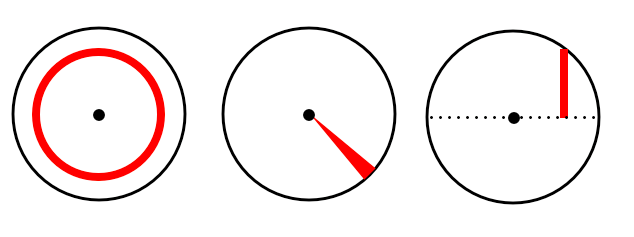
\includegraphics [scale=0.5] {circles3.png}\end{center}

Integration is used to compute areas and volumes, and other sums, by adding up many little pieces.  To calculate the area of a circle, we find the pieces we will use with one of three basic strategies:  rings, slices of pie, or rectangles of area underneath the function obtained by solving $x^2 + y^2 = R^2$ (using the positive square root).  These three approaches are illustrated in the figure above.

\subsection*{rings}
In the first approach (left panel), we imagine the area being computed by adding up the individual areas of a series of very thin, concentric rings.

The total area to be computed is that of a circle of a definite, fixed size, and we denote the radius of this circle by capital $R$, a constant.  On the other hand, the series of rings ranges from the origin of the circle to the circumference of the outmost ring.  Each one of this progression of rings has a radius, so we use the lowercase $r$ to describe them, with $r$ being a variable---$r$ varies from $0$ at the origin to $R$ at the outside of the circle.

Think about an individual ring, for example the outermost ring, which is similar to the circular peel or rind surrounding a thin slice of lemon.  We are working with areas here, in two dimensions, so the slice we imagine to be infinitely thin, and we are working with it as a cross-section or ring.

The area of the ring is the length times the width.  The length is the circumference, $2 \pi R$ for the outermost ring, but in general, for any of the inner rings it is $2 \pi r$. The length is multiplied by the width of the slice, which is a small element of radius, $dr$.  The small element of area contributed by an individual ring is $dA$:

\[ dA = 2 \pi r \ dr \]

Another way to explain this equation is to ask the question:

\textbf{how does area change with increasing radius}?  

If we take a circle and increase its radius by a little bit, how does the area change?  The answer is, it changes in proportion to the circumference, $2 \pi r$.

Another way to say the same thing is that the derivative is
\[ \frac{dA}{dr} = 2 \pi r \]

Proceeding from the first equation, the total area is the sum of the areas for the series of rings.

\[ A = \int dA = \int_0^R 2 \pi r \ dr \]

It's worth emphasizing how this view is different than the examples of integration one usually sees first in a calculus book:  these pieces of area are not rectangles but circles.  But it poses most clearly the question we are trying to answer, "how does area vary with $r$"?

The solution is
\[ \int_0^R 2 \pi r \ dr = 2 \pi \ \frac{1}{2}r^2 \ \bigg|_{r=0}^{r=R} = \pi R^2\]
as expected.  And we can check by differentiating:
\[ \frac{d}{dr} \ \pi r^2 = 2 \pi r \]

\subsection*{wedges}
\begin{center}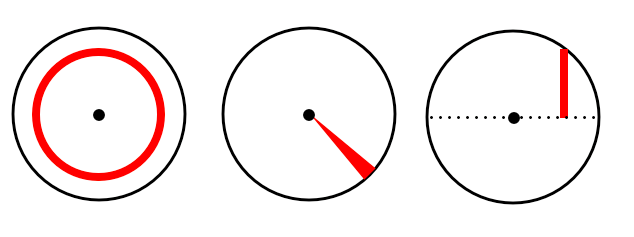
\includegraphics [scale=0.5] {circles3.png}\end{center}
In the second method (middle panel), we need to first find the area of a wedge.  For a thin enough slice, this is a triangle, with a familiar formula: one-half the base times the height.  The height is $R$, the radius of the circle.  

For the base we need the length of a piece of arc of a circle.  Recall that by definition, if we have a unit circle, then the angle of a wedge is equal to the arc it cuts out, and vice-versa, the arc is equal to the angle.  (Thus, the total length if we go all the way around the unit circle is $2 \pi$).  

For a circle with radius $R$, the length going all the way around is $2 \pi R$, and the length of arc for any angle $\theta$ is $\theta$ times $R$.

The area we want is built up of a series of wedges that are almost infinitely slender, with angle $d \theta$, so these wedges have bases measuring $R \ d \theta$.  The area of each triangular wedge is one-half the height times the base or
\[ dA = \frac{1}{2} R \ R \ d\theta \]

For the total area
\[ A = \int dA = \int  \frac{1}{2} R \ R \ d\theta \]
\[= \frac{1}{2} R^2 \int_{\theta=0}^{\theta=2\pi} \ d\theta \]
\[ = \frac{1}{2} R^2 \theta \  \bigg|_{\theta=0}^{\theta=2\pi} \]
\[ =  \pi R^2 \]

\subsection*{area under the curve}
\begin{center}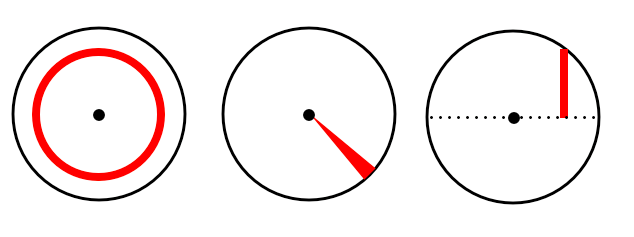
\includegraphics [scale=0.5] {circles3.png}\end{center}

The third view (right panel) is the most familiar, but has a somewhat harder calculation.  We want the area under the positive square root in the equation for a circle (right panel).
\begin{center}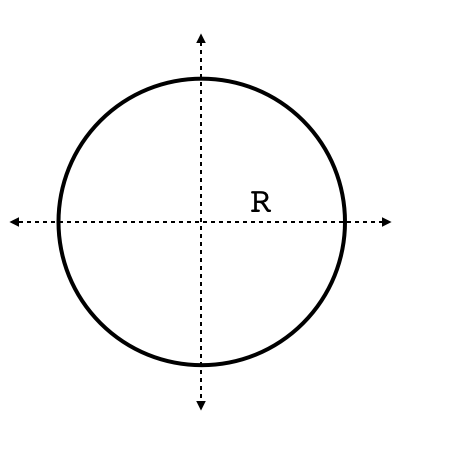
\includegraphics [scale=0.25] {circle.png}\end{center}

\[ x^2 + y^2 = R^2\]
\[ y = f(x) = \sqrt{R^2-x^2} \] 

To get the area, we need to integrate:
\[ \int y \ dx = \int_{-R}^{R} \sqrt{R^2-x^2} \ dx \]

but we don't have $x$ on top of that square root, so we can't do it directly.  We will work through this problem \hyperref[sec:Cosine_squared]{\textbf{later}}, after we review a few more techniques that are useful in doing integration problems.  

Of course, the answer will turn out to be just what you'd expect:
\[ A = \pi R^2 \]

\subsection*{Volume of the sphere}
We think about how the volume of the sphere depends on $r$ ($r = 0 \rightarrow R$).  An incremental change $dr$ changes the volume by adding a thin shell of volume equal to the surface area of the sphere ($4 \pi r^2$) times $dr$.  That is

\[ dV = 4 \pi r^2 \ dr \]
\[ V = \int dV = \int_0^R 4 \pi r^2 \ dr \]
\[ = 4 \pi \ \ \frac{1}{3}r^3 \ \bigg |_0^R = \frac{4}{3}\pi R^3 \]

It's really as simple as that.  Of course, you need to know the formula for the surface area to do it that way.  Alternatively, if you know the volume of the sphere, this is an easy way to get a formula for the surface area.

The image shows a "spherical lune", or segment of the surface of the sphere, as an aid to visualizing the whole surface.
\begin{center} 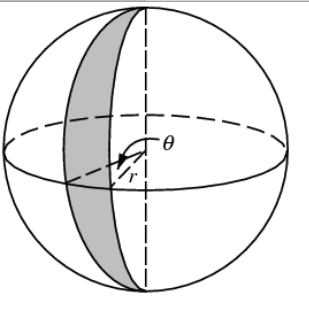
\includegraphics [scale=0.5] {spherical_lune.png} \end{center}
We'll say a lot more about the volume of the sphere \hyperref[sec:Volume_of_the_sphere]{\textbf{later}}. 

To make this even more concrete, here is a third example, to calculate the volume of a cone.  

\subsection*{volume of a cone}

We lay a cone along the $x$-axis with its vertex at the origin, opening to the right.
\begin{center}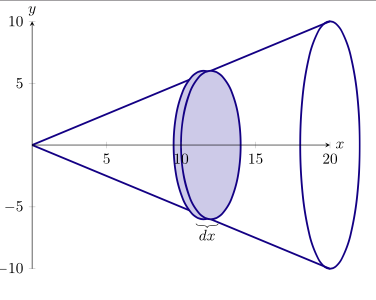
\includegraphics [scale=0.4] {cone_sideways.png}\end{center}
The cone is three-dimensional with the third axis ($z$) coming up out of the page.  The intersection with the $xy$-plane is a triangle.  

Can you see that in the $xy$-plane $y$ is a linear function of $x$, i.e. $y = kx$ where $k$ is a constant.  (The constant $k$ is actually the ratio of the radius $R$ to the height $H$.  That is equal to $\Delta y/\Delta x$.).
\[ y = \frac{R}{H} x \]

If we slice the cone into thin sections perpendicular to the $x$-axis, each little piece is a circle with radius $y$ and area $\pi y^2$.  For a thin enough slice, the volume is that area times the width of the slice:
\[ dV = \pi y^2 \ dx \]
Finding the volume of an individual piece is the important part of the calculus argument.

Now we just substitute the value of $y$ in terms of $x$
\[ dV = \pi \ [ \frac{R}{H} ]^2  x^2 \ dx \]
add up all the little volumes by setting up the integral
\[ V = \int dV = \int \pi \ [ \frac{R}{H} ]^2 x^2 \ dx \]

We apply a basic rule that constant terms can move "out from under" the integral sign:
\[ = \pi \ [ \frac{R}{H} ]^2 \ \int x^2 \ dx \]

We recognize that the value $x$ lies in the interval $[0,H]$ so these are the "bounds" on the integral
\[ = \pi \ [ \frac{R}{H} ]^2 \int_0^H x^2 \ dx \]

and then just follow the rule for doing a problem like this:  $\int x^2 = x^3/3$.  So
\[ = \pi \ [ \frac{R}{H} ]^2 \ [  \frac{x^3}{3} ] \ \bigg |_0^H \]
\[ = \frac{1}{3} \pi R^2 H \]

Once again, we obtain the formula of one-third times the area of the base times the height.  No matter what the shape of the base is, the area of each slice will be proportional to $x^2$ and we will end up with a formula involving one-third at the end.

We will see several other methods for obtaining this result.

We also note that we can obtain the volume of a fustrum (a cone whose top has been amputated) as
\[ = \pi \ [ \frac{R}{H} ]^2 \ [  \frac{x^3}{3} ] \ \bigg |_{h_1}^{h_2} \]
\[ = \pi \ [ \frac{R}{H} ]^2 \ [  \frac{{h_2}^3}{3} -  \frac{{h_1}^3}{3}  \ ] \]

\end{document}